\documentclass[]{beamer}


\usepackage[utf8]{inputenc}
\usepackage[percent]{overpic}
\usepackage{xcolor}
\usepackage{tcolorbox}
\usepackage[absolute,overlay]{textpos}
\usepackage{amsmath}
\usepackage{algorithmic}
\usepackage{algorithm}
\usepackage[english]{babel}

\usepackage{graphicx}
\usepackage{paralist}
\usepackage{setspace}
\usepackage{amsfonts}
\usepackage[labelfont=bf]{caption}
\usepackage{hyperref}
\usepackage{amssymb}
\usepackage{float}
\usepackage{placeins}
\usepackage{booktabs}
\usepackage{verbatim}
\usepackage{color,array}
\usepackage{colortbl}
\usepackage{lscape}
\usepackage{url}
\usepackage{centernot}
\usepackage{xfrac}
\newcommand{\fsl}[1]{{\centernot{#1}}}
\newcommand{\defgl}{\mathrel{=\!\!\mathop:}}
\newcommand{\defgr}{\mathrel{\mathop:\!\!=}}
\def\SM{{\rm SM}}
\def\NP{{\rm NP}}
\def\ubar{\overline{u}}
\def\dbar{\overline{d}}
\def\sbar{\overline{s}}
\def\cbar{\overline{c}}
\def\bbar{\overline{b}}
\def\tbar{\overline{t}}
\def\qbar{\overline{q}}
\def\lbar{\overline{\ell}}
\def\ebar{\overline{e}}
\def\mubar{\overline{\mu}}
\def\nubar{\overline{\nu}}
\def\Qbar{\overline{Q}}
\def\Lbar{\overline{L}}
\def\ml{{{m_\ell}}}
\def\Babar{{\mbox{\slshape B\kern-0.1em{\smaller A}\kern-0.1em B\kern-0.1em{\smaller A\kern-0.2em R}}}}

\DeclareMathOperator{\Tr}{Tr}
\newcommand{\nn}{\nonumber}


\definecolor{tugreen}{HTML}{990000}
\definecolor{tugrey}{HTML}{990000}
\definecolor{tured}{HTML}{990000}
\setbeamercolor{palette compare}{bg=white!80!tugreen,fg=black}
\setbeamercolor{palette misc}{bg=white!80!tugreen,fg=black}
\setbeamercolor{palette white}{bg=white!99!black,fg=black}


\makeatletter
\renewcommand{\itemize}[1][]{%
  \beamer@ifempty{#1}{}{\def\beamer@defaultospec{#1}}%
  \ifnum \@itemdepth >2\relax\@toodeep\else
    \advance\@itemdepth\@ne
    \beamer@computepref\@itemdepth% sets \beameritemnestingprefix
    \usebeamerfont{itemize/enumerate \beameritemnestingprefix body}%
    \usebeamercolor[fg]{itemize/enumerate \beameritemnestingprefix body}%
    \usebeamertemplate{itemize/enumerate \beameritemnestingprefix body begin}%
    \list
      {\usebeamertemplate{itemize \beameritemnestingprefix item}}
      {\setlength\itemsep{0.7em}% NEW
        \def\makelabel##1{%
          {%
            \hss\llap{{%
                \usebeamerfont*{itemize \beameritemnestingprefix item}%
                \usebeamercolor[fg]{itemize \beameritemnestingprefix item}##1}}%
          }%
        }%
      }
  \fi%
  \beamer@cramped%
  \raggedright%
  \beamer@firstlineitemizeunskip%
}
\makeatother

\newcommand{\backupbegin}{
	\newcounter{finalframe}
	\setcounter{finalframe}{\value{framenumber}}
}
\newcommand{\backupend}{
	\setcounter{framenumber}{\value{finalframe}}
}


\mode<presentation>
{ \usetheme[color=green]{TU_Dortmund}
}



\title{\Large SQuIDS: A Tool to Solve Time Evolution in finite dimensional (open) Quantum Systems\\\vspace*{0.5cm}{\small An Application to Neutrino Oscillations\\\href{https://arxiv.org/abs/1412.3832.pdf}{arxiv:1412.3832}}}
\author{Dominik Hellmann}
\institute[TU Dortmund]{\scriptsize TU Dortmund\\WG Päs
}

\date{May 3, 2023}

\begin{document}
\nocite{*}


\frame{\titlepage}

\begin{frame}
  Outline:
  \begin{enumerate}
    \item Introduction (Quantum Evolution with Density Matrices)
    \item SQuIDS (Overview and Exercises)
    \begin{enumerate}
      \item The Const class (Overview + Exercise)
      \item The SU\_vector class (Overview + Exercise)
      \item The SQuIDS class (Overview + Exercise)
    \end{enumerate}
  \end{enumerate}
\end{frame}

\section{Introduction}

\begin{frame}{Motivation}
  Task: Solve time evolution of finite dimensional quantum (sub-)systems:
  \begin{itemize}
    \item Flavor oscillations
    \item Quantum computation
    \item Systems with finitely many energy levels
    \item Spins
  \end{itemize}
  Time evolution of closed quantum system: Schrödinger equation
  \begin{align}
    i \frac{\partial}{\partial t} \vert \psi \rangle &= \hat{H} \vert \psi \rangle \qquad (\hbar = 1)
  \end{align} 
\end{frame}

\begin{frame}{Density matrices instead of state vectors}
  Often: finite dimensional system \(S\) coupled to a complicated (but uninteresting) environment \(E\)
  \begin{itemize}
    \item[\(\rightarrow\)] Get rid of Environment (keyword: partial trace)
    \item[\(\rightarrow\)] Just consider degrees of freedom of interest
  \end{itemize}
  \textbf{Consequence: Decoherence}
  \begin{itemize}
    \item Subsystem cannot be described by pure state \(\vert \psi \rangle\)
    \item Mixed state: Described by density matrix \(\varrho = \sum_{i} p_i \vert \psi_i \rangle \langle \psi_i \vert\)
  \end{itemize}
\end{frame}

\begin{frame}{Example: Neutrino oscillations in matter}
  \begin{center}
    \begin{tabular}[t]{c|c}
      \(S \simeq \mathbb{C}^3\) & \(E\) \\
      \toprule
      flavor degrees of freedom & all remaining d.o.f (momenta, spins, \ldots) \\
      \(\vert \psi \rangle = \sum_{\alpha = e}^{\tau}\psi_\alpha \vert \nu_\alpha \rangle \) & \(\rightarrow\) infinite dimensional 
    \end{tabular}
  \end{center}
  \vspace{0.5cm}
  \begin{itemize}
    \item We are not at all interested in \(E\)
    \item Only the \(\nu\) flavor composition is interesting to us 
    \item \textbf{But}: \(E\) significantly influences flavor d.o.f.
  \end{itemize}
  \(\Rightarrow\) Need effective description!
\end{frame}

\begin{frame}{Time evolution of the density matrix}
  Master equation(s): (multiple density matrices possible)
  \begin{align*}
    \frac{\mathrm{d}\varrho_j}{\mathrm{d}t} &= -i [\hat{H}_j(t), \varrho_j(t)] + \{\Gamma_j(t), \varrho_j(t)\} + F_j[\{\varrho_k\}_k, t]
  \end{align*}
  \begin{itemize}
    \item Why multiple \(\varrho_j\)? E.g.: One per energy bin!
    \item \(\hat{H} = \hat{H}_0 + \hat{H}_1(t)\): Unitary evolution
    \item \(\Gamma\): Decoherence
    \item \(F\): Other non-linear effects (coupling between \(\varrho_j\))
  \end{itemize}
\end{frame}

\begin{frame}{Simple Example: \(\nu\) Oscillations in Vacuum}
  Neutrino Experiment:
  \begin{columns}
    \begin{column}{0.5\textwidth}
      \begin{itemize}
        \item Fixed baseline \(L\)
        \item \(N\) energy bins \(\{E_j\}_j\)
        \item \(\hat{H}^j = \hat{H}_0^j = E_j \cdot \mathbb{I} + \frac{1}{2E_j} \mathbb{M}^2\)
        \item \(\Gamma \equiv 0\)
        \item \(F \equiv 0\)
        \item \(\varrho_j(t) = \sum_{\alpha = e}^{\tau} \phi_{\alpha}^j(t) \vert \nu_\alpha \rangle \langle \nu_\alpha \vert\)
      \end{itemize}
    \end{column}
    \begin{column}{0.5\textwidth}
      \begin{align*}
        \mathbb{M} &= \sum_{j, k = 1}^{3} (\mathbb{M}_{0})_{jk} \vert \nu_j \rangle \langle \nu_k \vert \\
        &= \sum_{\alpha, \beta = e}^{\tau} (\mathbb{M}_{1})_{\alpha\beta} \vert \nu_\alpha \rangle \langle \nu_\beta \vert \\
        \mathbb{M}_{0} &= \begin{pmatrix}
          m_1 & 0 & 0 \\
          0 & m_2 & 0 \\
          0 & 0 & m_3
        \end{pmatrix} \\
        \mathbb{M}_{1} &= U_{\mathrm{PMNS}}^\dagger \mathbb{M}_{0} U_{\mathrm{PMNS}}
      \end{align*}
    \end{column}
  \end{columns}
\end{frame}

\begin{frame}{Some Important Considerations}
  The master equation simplifies to
  \begin{align*}
    \frac{\mathrm{d}\varrho_j}{\mathrm{d}t} &= -i [\hat{H}_0^j, \varrho_j(t)]
  \end{align*}
  Further simplifications
  \begin{itemize}
    \item Consider in mass basis: \(\hat{H}_0^j\) is diagonal
    \item Depends only on commutator!
    \begin{itemize}
      \item \([A, \mathbb{I}] = 0\) \(\Rightarrow\) \([\hat{H}_0^j, \varrho_j(t)] = [\hat{H}_0^j - \epsilon_j \mathbb{I}, \varrho_j(t)]\)
      \item \(\epsilon_j := E_j + \sfrac{m_1^2}{2 E_j}\)
    \end{itemize}
  \end{itemize}
  \begin{align*}
    \tilde{H}^j &= \frac{1}{2E_j}\begin{pmatrix}
      0 & 0 & 0 \\
      0 & \Delta m_{21}^2 & 0 \\
      0 & 0 & \Delta m_{31}^2 
    \end{pmatrix}
  \end{align*}
\end{frame}

\begin{frame}{Some Important Considerations (ctd.)}
  Can solve \(H_0\) evolution analytically!
  \begin{itemize}
    \item Pass to interaction picture:
    \begin{align*}
      \tilde{\varrho}(t) &:= \exp(i H_0 t) \varrho \exp(-i H_0 t) \\
      \Rightarrow \dot{\varrho} &= - i [H_0, \rho] + \exp(-i H_0 t) \dot{\tilde{\varrho}} \exp(i H_0 t)
    \end{align*}
    \item Can subtract \(-i[H_0, \varrho]\) on both sides of master equation
    \item Must transform all terms to interaction picture (SQuIDS does that automatically and efficiently)
  \end{itemize}
\end{frame}

\begin{frame}{Some Important Considerations (ctd.)}
  All matrices in our system are hermitian: \(A^\dagger = A\)
  \begin{itemize}
    \item Hermitian \(n \times n\) matrices form \(N = n^2\) dimenional real vector space
    \item Convenient basis: \(SU(n)\) generators \(\sigma_i\) (e.g. \(n = 2\): Pauli matrices + identity)
    \item Decompose: \(\varrho = \sum_{i = 0}^{n^2 - 1} \rho_i \cdot \sigma_i\)
    \item Components \(\rho_i\) form \(n^2\) dimensional vector called \texttt{SU\_vector} in the following
  \end{itemize}
\end{frame}

\begin{frame}{Summary}
  What did we learn so far (in general):
  \begin{enumerate}
    \item We passed to density matrix formulation (allows for mixed states)
    \item Formulated master equation
    \item Can subtract \(\epsilon_0 \cdot \mathbb{I}\) from \(\hat{H}\) (only energy diff. important)
    \item Can solve \(\hat{H}_0\) exactly (interaction picture) \(\varrho \rightarrow e^{i\hat{H}_0 t} \varrho e^{- i\hat{H}_0 t}\)
    \item Can represent \(\varrho, H, \ldots\) as \(n^2\) dimensional, real vector (\texttt{SU\_vector})!
    \begin{itemize}
      \item[\(\rightarrow\)] Efficient and preserves hermiticity automatically!
    \end{itemize}
  \end{enumerate}
\end{frame}

\section{SQuIDS}

\begin{frame}
  \centering {\Huge SQuIDS}
\end{frame}

\begin{frame}{Clone the Repo!}
  Git Repository includes all needed files (slides, code templates)
  \begin{block}{Instructions}
    \texttt{cd} to the location where you want to place the repo \\
    \texttt{git clone https://github.com/B0bsen/sm\_to\_bsm\_neutrino.git} \\
    \texttt{cd sm\_to\_bsm\_neutrino}
  \end{block}
\end{frame}

\begin{frame}{Overview}
  SQuIDS mainly consists out of 3 interconnected classes:
  \begin{enumerate}
    \item<1-> \texttt{squids::Const}
    \begin{itemize}
      \item<1-> Implements all sorts of constants of nature
      \item<1-> Conversion between natural units and other unit systems
      \item<1-> Stores system parameters (mixing angles, energy differences, \ldots)
    \end{itemize} 
    \item<2-> \texttt{squids::SU\_vector}
    \begin{itemize}
      \item<2-> Represents hermitian matrices efficiently
      \item<2-> Implements all sorts of operations on them (Unitary transformations, trace, commutator, \ldots)
    \end{itemize}
    \item<3-> \texttt{squids::SQuIDS}
    \begin{itemize}
      \item<3-> Abstract base class, uses \texttt{squids::Const} and \texttt{squids::SU\_vector}
      \item<3-> Implements time evolution of the system of density matrices
      \item<3-> Includes methods for taking expectation values etc
    \end{itemize}
  \end{enumerate}
\end{frame}

\begin{frame}
  \centering {\Huge SQuIDS - The Const Class}
\end{frame}

\subsection{SQuIDS - Const}
\begin{frame}{Const - Construction of objects}
  Can only be default constructed:
  \begin{tcolorbox}[colback=gray!5!white]
    \texttt{squids::Const units;} 
  \end{tcolorbox}
  \begin{itemize}
    \item Constructs \texttt{squids::Const} object called \texttt{units}
    \item This object contains
    \begin{itemize}
      \item Different physical constants (\(G_F, N_A, G, m_{p}, \ldots\))
      \item Values of km, s, J, kg, etc. in natural units
      \item Yet unspecified values for: 
      \begin{itemize}
        \item basis change from \(B_0\) to \(B_1\) (e.g. mass and flavor basis)
        \item energy differences which can be used for the hamiltonian \(\hat{H}_0\)
      \end{itemize}
    \end{itemize}
  \end{itemize}
\end{frame}

\begin{frame}{Const -  Unit conversion}
  Easily convert between SI and natural units:
  \begin{tcolorbox}[colback=gray!5!white]
    \texttt{squids::Const units;} \\
    \texttt{double L = 10 * units.cm; \textcolor{olive}{\textbackslash \textbackslash {} 506773 eV\^{}\{-1\}}} \\ 
    \texttt{double T = 1 * units.year; \textcolor{olive}{\textbackslash \textbackslash {} 4.79116e+22 eV\^{}\{-1\}}} \\
    \texttt{double GF = units.GF * (units.GeV * units.GeV); \textcolor{olive}{\textbackslash \textbackslash {} 1.16638e-05 GeV\^{}\{-2\}}}
  \end{tcolorbox}
  The units are to be read as \texttt{[unit we want]} / \texttt{[eV}\(^{\alpha}\)\texttt{]}, e.g.:
  \begin{itemize}
    \item[\texttt{km} / \texttt{[eV}\(^{-1}\)\texttt{]}:] \texttt{[Value in eV}\(^{-1}\)\texttt{]} \(=\) \texttt{[Value in km]} \(\cdot\) \texttt{km} / \texttt{[eV}\(^{-1}\)\texttt{]}
  \end{itemize}
  \texttt{[Value in km]} \(= L \) / \texttt{km}
\end{frame}

\begin{frame}{Const -  Setting / Getting Mixing Angles}
  Furthermore you can store system parameters:
  \begin{tcolorbox}[colback=gray!5!white]
    \texttt{squids::Const params;} \\
    \textcolor{olive}{\texttt{\textbackslash \textbackslash {} Sets} \(\theta_{12} = 24\)°} \\
    \texttt{params.SetMixingAngle(0, 1, 24 * params.degree);} \\
    \textcolor{olive}{\texttt{\textbackslash \textbackslash {} Sets} \(\delta_{13} = 2\)°} \\
    \texttt{params.SetPhase(0, 2, 2 * params.degree);} \\
    \textcolor{olive}{\texttt{\textbackslash \textbackslash {} Sets} \(\Delta E_{10} = 7 \mathrm{eV}\)} \\
    \texttt{params.SetEnergyDifference(1, 7 * params.eV);}
  \end{tcolorbox}
  \begin{itemize}
    \item Substitute \texttt{Set} for \texttt{Get}: returns corresponding value
    \item Energy differences: Only convenience parameters simplifying definition of \(\hat{H}_0\)
  \end{itemize}
\end{frame}

\subsection{SQuIDS - Const: Exercise}

\begin{frame}
  \centering {\Huge SQuIDS - The Const Class: Exercise}
\end{frame}

\begin{frame}{Const class exercise}
  \begin{enumerate}
    \item Declare a default constructed const class object
    \item Answer the following questions:
    \begin{enumerate}
      \item How many \(\mathrm{eV}^{-1}\) correspond to \(300\,\mathrm{km}\)
      \item How many radians correspond to \(25^\circ\)
      \item If you are \(24\) years old, how many \(eV^{-1}\) are you old?
    \end{enumerate}
    \item Set the mixing parameters for three neutrino generations to:
    \begin{itemize}
      \item \(\theta_{12} = 33.48^\circ\)
      \item \(\theta_{13} = 8.55^\circ\)
      \item \(\theta_{23} = 42.3^\circ\)
    \end{itemize}
    \item Set the energy differences to:
    \begin{itemize}
      \item \(\Delta m^2_{21} = 7.5 \cdot 10^{-5} \, \mathrm{eV}^2\)
      \item \(\Delta m^2_{31} = 2.45 \cdot 10^{-3} \, \mathrm{eV}^2\)
    \end{itemize}
  \end{enumerate}
\end{frame}

\subsection{SQuIDS - SU\_vector}

\begin{frame}
  \centering {\Huge SQuIDS - The SU\_vector Class}
\end{frame}

\begin{frame}{SU Vector - Contructors}
  Construct a SU Vector:
  \begin{itemize}
    \item Default: No entries, no size
    \begin{tcolorbox}[colback=gray!5!white]
      \texttt{squids::SU\_vector rho;}
    \end{tcolorbox}
    \item Defined Dimension: entries are zero, size is \texttt{dim}(\(\mathcal{H}\))\(> 0\)
    \begin{tcolorbox}[colback=gray!5!white]
      \texttt{squids::SU\_vector rho(dim); \textcolor{olive}{\textbackslash \textbackslash size = dim}\(^2\)}
    \end{tcolorbox}
  \end{itemize}
  And more: construct from \texttt{array}, \texttt{gsl\_matrix\_complex}, \texttt{std::vector} \ldots
\end{frame}

\begin{frame}{SU Vector - Special Matrices}
  Construct a SU Vector to Standard Form:
  \begin{itemize}
    \item Identity: Corresponding matrix is the identity \((Id)_{ij} = \delta_{ij}\)
    \begin{tcolorbox}[colback=gray!5!white]
      \texttt{squids::SU\_vector Id }\\
      \texttt{= squids::SU\_vector::Identity(dim);}
    \end{tcolorbox}
    \item Projector on state \(k_0\): only the \((k_0,k_0)\) element is 1, i.e. \((\mathbb{P}_{k_0})_{ij} = \delta_{i k_0} \delta_{j k_0}\)
    \begin{tcolorbox}[colback=gray!5!white]
      \texttt{squids::SU\_vector P\_k0} \\
      \texttt{= squids::SU\_vector::Projector(dim, k0);}
    \end{tcolorbox}
  \end{itemize}
  And more: See \href{https://arxiv.org/abs/1412.3832}{documentation} (also in the repo)
\end{frame}

\begin{frame}{SU Vector - Functions}
  Manipulate a SU Vector:
  \begin{itemize}
    \item Rotate from one basis to another (\(B_0 \leftrightarrow B_1\)): (using angles specfied in params)
    \begin{tcolorbox}[colback=gray!5!white]
      \texttt{rho.RotateToB1(params); \textcolor{olive}{\textbackslash \textbackslash B0 to B1}} \\
      \texttt{rho.RotateToB0(params); \textcolor{olive}{\textbackslash \textbackslash B1 to B0}}
    \end{tcolorbox}
    \item Return dim of Hilbert space, Size of vector:
    \begin{tcolorbox}[colback=gray!5!white]
      \texttt{rho.Dim(); \textcolor{olive}{\textbackslash \textbackslash returns dim(H)}} \\
      \texttt{rho.Size(); \textcolor{olive}{\textbackslash \textbackslash returns number of elements}}
    \end{tcolorbox}
  \end{itemize}
  Furthermore: You can add, subtract multiply (also with scalars), assign, access elements via \texttt{rho[]} etc.
\end{frame}

\subsection{SQuIDS - SU\_vector: Exercise}

\begin{frame}
  \centering {\Huge SQuIDS - The SU\_vector Class: Exercise}
\end{frame}

\begin{frame}{SU vector exercise}
  \begin{enumerate}
    \item Declare an empty SU vector corresponding to a 3D Hilbert space
    \item Initialize an array of projectors for the three mass eigenstates (\(B_0\))
    \item Rotate them to the flavor basis (\(B_1\))
    \item Initialize a SU vector corresponding to the matrix (\(B_0\))
    \begin{align}
      \Delta \mathbb{M}^2 := \begin{pmatrix}
        0 & 0 & 0 \\
        0 & \Delta m_{21}^2 & 0 \\
        0 & 0 & m_{31}^2 \\
      \end{pmatrix}
    \end{align}
  \end{enumerate}
\end{frame}

\subsection{SQuIDS - SQuIDS}

\begin{frame}
  \centering {\Huge SQuIDS - The SQuIDS Class}
\end{frame}

\begin{frame}{SQuIDS - General Overview pt. I}
  \texttt{squids::SQuIDS} is a so called base class:
  \begin{itemize}
    \item You derive your own class from it 
    \item It provides fundamental functionality through member functions
    \begin{itemize}
      \item Integration of the master equation
      \item Efficient memory management and storage of density matrices
    \end{itemize}
    \item Already includes several members storing basic data of your system 
    \item Virtual member functions:
    \begin{itemize}
      \item Some you have to define for the class to work (\texttt{H0}, constructors, \texttt{init}, \ldots)
      \item Some you can ignore if your system doesn't need them
    \end{itemize}
  \end{itemize}
\end{frame}

\begin{frame}{SQuIDS - General Overview pt. II}
  Distribution of density matrices across the nodes [arxiv:1412.3832]:
  \begin{center}
    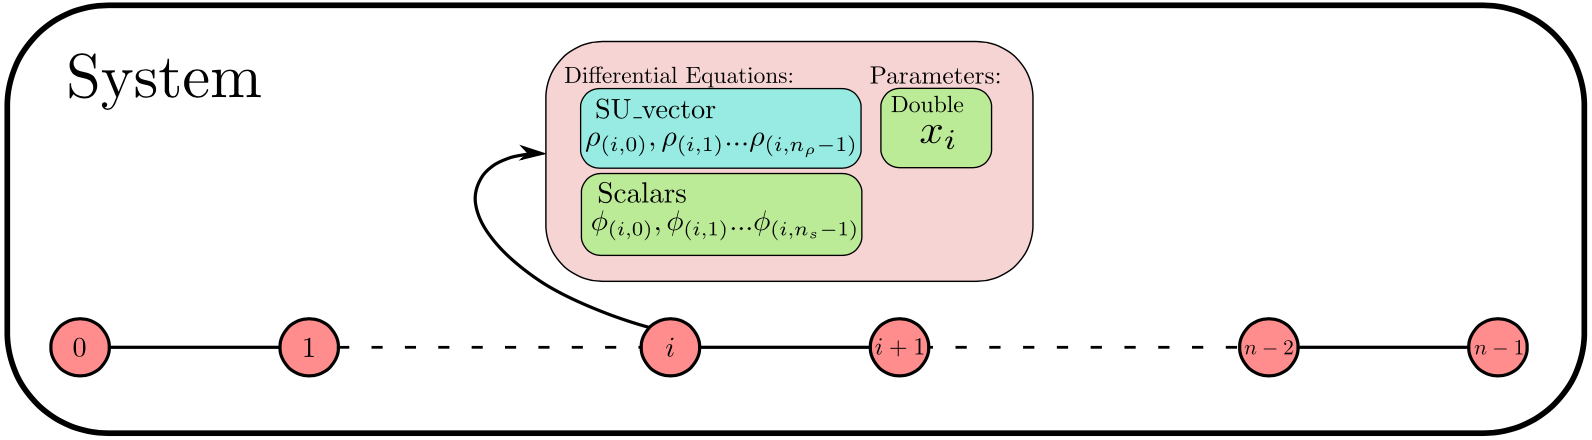
\includegraphics[width=0.8\textwidth]{figs/squids_nodes.png}
  \end{center}
  \begin{itemize}
    \item \texttt{n} nodes \(x_i\) (energy bins, angles, whatever feature of your system)
    \item At each node:
    \begin{itemize}
      \item \texttt{nrho} density matrices
      \item \texttt{ns} scalars (not important for us)
    \end{itemize}
  \end{itemize}
  \(\rightarrow\) Specify initial data, \texttt{H0}, \texttt{HI}, \texttt{GammaRho}, etc. \\
  \(\Rightarrow\) \texttt{SQuIDS} evolves the whole system (+ can take expectation values of observables)
\end{frame}

\begin{frame}{SQuIDS - Constructors}
  Constructors / Initializors: (Set bkg. params and allocate memory)
  \begin{tcolorbox}[colback=gray!5!white]
    \texttt{SQuDIS(); \textcolor{olive}{\textbackslash\textbackslash {} default}} \\
    \texttt{SQuDIS(uint nx, uint dim, unit nrho, uint nscalar, double ti = 0);} \\
    \texttt{void ini(uint nx, uint dim, unit nrho, uint nscalar, double ti = 0);}
  \end{tcolorbox}
  \begin{itemize}
    \item \texttt{nx}: Number of \(x\) nodes \texttt{x\_i}
    \item \texttt{dim}: Dimensions of Hilbert space
    \item \texttt{nrho} / \texttt{nscalar}: \# density matrices / scalars \emph{per node}
    \item \texttt{ti}: initial time, defaults to zero
  \end{itemize}
  \textbf{Call them in your own constructor with the system parameters you need!}
\end{frame}

\begin{frame}{SQuIDS - Member variables}
  SQuIDS is set up to include the following member variables:
  \begin{itemize}
    \item \texttt{std::vector<double> x}: \(x\) range
    \item \texttt{uint nsun}: Dim. of Hilbertspace
    \item \texttt{Const params}: \texttt{squids::Const} object containing system parameters
    \item And many more!
  \end{itemize}
  You can (and should) access these from within your own member functions!
\end{frame}

\begin{frame}{SQuIDS - Handy functions}
  Some very useful predefined member functions are:
  {\small\begin{tcolorbox}[colback=gray!5!white]
    \uncover<1->{\texttt{int Set\_xrange(double xini, double xend, std::string scale); \textcolor{olive}{\textbackslash\textbackslash {} Sets x = \{xini, \ldots, xend\} with lin or log scale}}} \\
    \uncover<2->{\texttt{double Get\_x(uint i) const; \textcolor{olive}{\textbackslash\textbackslash {} Returns x[i]}}} \\
    \uncover<3->{\texttt{const * Const Get\_params() const; \textcolor{olive}{\textbackslash\textbackslash {} Returns Const member}}} \\
    \uncover<4->{\texttt{int Evolve(double dt); \textcolor{olive}{\textbackslash\textbackslash {} Evolves System by dt}}} \\
    \uncover<5->{\texttt{double GetExpectationValue(SU\_vector op, uint irho, uint ix) const; \textcolor{olive}{\textbackslash\textbackslash {} Calculates exp. val. of op at node ix with density matrix irho at current time}}}
  \end{tcolorbox}}
  \uncover<6->{Of course there are more but these are most important for us!}
\end{frame}

\begin{frame}{SQuIDS - Evolution functions}
  Last but not least: The time independent Hamiltonian \texttt{H0}
  \begin{tcolorbox}[colback=gray!5!white]
  \texttt{SU\_vector H0(double x, uint irho) const;}
  \end{tcolorbox}
  \begin{itemize}
    \item Returns \(\hat{H}_0\) as \texttt{SU\_vector} object
    \item Assumes that \(\hat{H}_0\) diagonal (i.e. given in mass basis \texttt{B0} for \(\nu\) oscillations)
    \item Cannot modify but can read member variables (const)
    \item \texttt{irho}: \texttt{H0} for density matrix at node \(x_i\)
  \end{itemize}
\end{frame}

\subsection{SQuIDS - SQuIDS: Exercise}

\begin{frame}
  \centering {\Huge SQuIDS - The SQuIDS Class: Exercise}
\end{frame}

\begin{frame}{SQuIDS application: Neutrino oscillations in vacuum}
  General set up: Vacuum Oscillations Experiment with \ldots
  \begin{itemize}
    \item Fixed baseline \(L\) (\(\hat{=}\) time variable)
    \item \texttt{n} logarithmic energy bins: \(E \in [10\,\mathrm{MeV}, 10\,\mathrm{GeV}]\)
    \item All neutrinos are produced as electron neutrinos
  \end{itemize}
  Use: \texttt{x} nodes as energy nodes, one density matrix per node, no scalar functions, only \texttt{H0} non-zero
\end{frame}

\begin{frame}{SQuIDS application: Neutrino oscillations in vacuum}
  \begin{enumerate}
    \item Declare vacuum class publically derived from squids::SQuIDS class in \texttt{vac/src/vacuum.hpp} with methods
    \begin{itemize}
      \item Default constructor
      \item Initializing constructor
      \item \texttt{H0}
      \item \texttt{GetProbabilities}
      \item Destructor if needed
    \end{itemize}
    \item Define the corresponding member functions in \texttt{vac/src/vacuum.cpp}
    \begin{itemize}
      \item \texttt{nbins} \(x\)-nodes corresponding to number of \(E\) bins (log scaled)
      \item One density function per node, no scalar functions
      \item \texttt{nflavor} neutrino flavors
      \item Initial condition \(\varrho_i(t = 0) = \mathbb{P}_{e}\) for all \(i \in \{1, \ldots,\texttt{nbins}\}\)
      \item Work in mass basis!!!
    \end{itemize}
  \end{enumerate}
\end{frame}

\begin{frame}{SQuIDS application: Neutrino oscillations in vacuum}
  \begin{enumerate}
    \setcounter{enumi}{2}
    \item Initialize an object from your class in \texttt{vac/src/main.cpp} (\texttt{nbins} = 1000, \texttt{nflavor} = 3, \(E \in [10 \,\mathrm{MeV}, 10 \,\mathrm{GeV}]\))
    \item Evolve the system for \(L = 300 \; \mathrm{km}\)
    \item Save the oscillation probabilities \(P_{e\alpha}(E_j, L)\) to file(s) \(\alpha = e, \mu, \tau\)
    \item Plot them against the energy
  \end{enumerate}
\end{frame}

\begin{frame}{Outlook}
  \begin{itemize}
    \item So far we only scratched the surface of SQuIDS' abilities
    \item Including \(\hat{H}_1(t), \Gamma, F \neq 0\) opens up possibilities to solve a vast range of systems
  \end{itemize}
\end{frame}

\appendix

\section{Backup}
\backupbegin

\begin{frame}
    \centering \Huge BACK UP
\end{frame}

\begin{frame}{Installation}
  What do we need for this tutorial?
  \begin{itemize}
    \item A unix-like (sub-)system 
    \begin{itemize}
      \item Linux
      \item Mac (+ Xcode developer tools!)
      \item On Windows: WSL
    \end{itemize}
    \item A C++ compiler
    \item Make, wget, Git
  \end{itemize}
  Use scripts \texttt{install\_gsl.sh} and \texttt{install\_SQuIDS.sh} from the repo!
\end{frame}

\begin{frame}{Installation (GSL)}
  \begin{columns}
    \begin{column}{\textwidth}
      {\tiny
        \begin{tcolorbox}[colback=gray!5!white]
        \texttt{cd \$HOME} \\
        \texttt{mkdir -p smToBsmLibs/gsl} \\
        \texttt{wget ftp://ftp.gnu.org/gnu/gsl/gsl-latest.tar.gz} \\
        \texttt{tar -zxvf gsl-latest.tar.gz} \\
        \texttt{rm gsl-latest.tar.gz} \\
        \texttt{cd \$(find gsl-* | head -n 1)} \\
        \texttt{./configure --prefix=\$HOME/smToBsmLibs/gsl} \\
        \texttt{make} \\
        \texttt{make check} \\
        \texttt{make install} \\
        \texttt{LD\_LIBRARY\_PATH=\$HOME/smToBsmLibs/gsl/lib:\$LD\_LIBRARY\_PATH} \\
        \texttt{export LD\_LIBRARY\_PATH} \\
        \texttt{cd \$HOME} \\
        \texttt{rm -rf \$(find gsl-* | head -n 1)}
      \end{tcolorbox}}
    \end{column}
  \end{columns}
\end{frame}

\begin{frame}{Installation (SQuIDS)}
  \begin{columns}
    \begin{column}{\textwidth}
      {\tiny
        \begin{tcolorbox}[colback=gray!5!white]
        \texttt{cd \$HOME} \\
        \texttt{mkdir -p smToBsmLibs/SQuIDS} \\
        \texttt{git clone https://github.com/jsalvado/SQuIDS.git} \\
        \texttt{cd \$(find SQuIDS* | head -n 1)} \\
        \texttt{./configure --with-gsl-incdir=\$HOME/smToBsmLibs/gsl/include \textbackslash} \\
        \texttt{  --with-gsl-libdir=\$HOME/smToBsmLibs/gsl/lib \textbackslash} \\ 
        \texttt{  --prefix=\$HOME/smToBsmLibs/SQuIDS} \\
        \texttt{make} \\
        \texttt{make test} \\
        \texttt{make install} \\
        \texttt{LD\_LIBRARY\_PATH=\$HOME/smToBsmLibs/SQuIDS/lib:\$LD\_LIBRARY\_PATH \textcolor{olive}{\# linux only}} \\
        \texttt{export LD\_LIBRARY\_PATH \textcolor{olive}{\# linux only}} \\
        \texttt{cd \$HOME} \\
        \texttt{rm -rf \$(find SQuIDS* | head -n 1)}
      \end{tcolorbox}}
    \end{column}
  \end{columns}
\end{frame}

\backupend

\end{document}
